\documentclass[12pt]{article}
\usepackage{graphicx}
\usepackage{url}

% The following parameters seem to provide a reasonable page setup.
\topmargin 0.0cm
\oddsidemargin 0.2cm
\textwidth 16cm 
\textheight 21cm
\footskip 1.0cm


%The next command sets up an environment for the abstract to your paper.
\newenvironment{sciabstract}{%
\begin{quote} \bf}
{\end{quote}}

\newcounter{lastnote}
\newenvironment{scilastnote}{%
\setcounter{lastnote}{\value{enumiv}}%
\addtocounter{lastnote}{+1}%
\begin{list}%
{\arabic{lastnote}.}
{\setlength{\leftmargin}{.22in}}
{\setlength{\labelsep}{.5em}}}
{\end{list}}


\title{Using Markov Chains to Manage Resource Gathering, Base Building \& Unit Building in StarCraft\hspace{4cm}\\
\line(1, 0){300}
} 
\author
{\textit{Giovanni Campo, Patrick O'Halloran \& Jeremiah Dunn}\vspace{0.3cm}\\\vspace{0.2cm}\line(1, 0){300}}
\date{}


\begin{document} 

% Double-space the manuscript.
\baselineskip24pt


% Make the title.
\maketitle 



% Place your abstract within the special {sciabstract} environment.

\begin{sciabstract}
 	This paper will discus an implementation the implementation of certain aspects of an AI controller which could be used in the Student StarCraft AI Tournament (SSCAI).\cite{sscai} The implementation will focus on the use of Markov chains to manage recourse gathering.
\end{sciabstract}


\section{Introduction}

-Student StarCraftAI tournament.

-overview of our proposal, what we hope to achieve

\begin{figure}
\centering
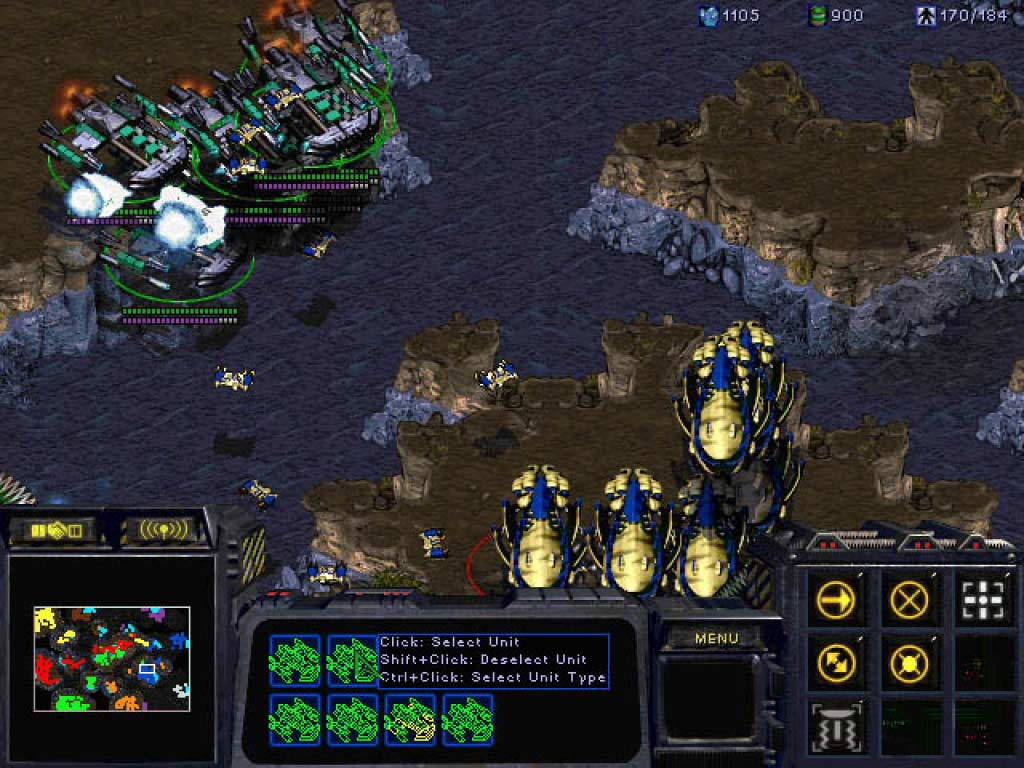
\includegraphics[scale=0.4, trim = 0cm 0cm 0cm 0cm]{images/test}
\label{fig:test}
\caption{some figure}
\end{figure}

\subsection{Making sure this works ok}

some subsection paragraph some subsection paragraph some subsection paragraph some subsection paragraph some subsection paragraph some subsection paragraph some subsection paragraph

check out figure~\ref{fig:test}

whoa, a reference~\cite{gershenfeld1999nature}


\section{Markov Chains}

Markov chains are weighted finite state machines.

%move to intro section?

-what are Markov chains

-how have they been used with starcraft before

-what is our motivation for using them with our bot


\section{Implementation}

\subsection{SCV Units}

The \textit{Terran} race uses SCV units to harvest resources and build structures. At the start of a game there are four SCVs available to the player.

Figure~\ref{fig:scv_diagram} shows the Markov Chain which dictates the behaviour of the SCV units. The transition from Building to Idle has no probability assigned to it. Building is taken to be a distinct state but exiting the state is controlled by the game, not the agent. The probabilities \(P_{IB}\) and \(P_{IH}\) refer to the probability that an idle agent will chose to start harvesting or to start building. \(P_{HB}\) refers to the probability of a harvesting agent stopping and beginning building.

\begin{figure}
\centering
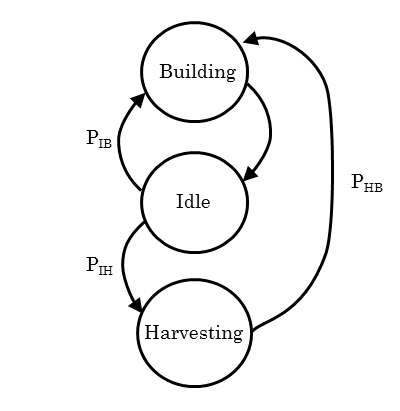
\includegraphics[scale=0.8, trim = 0cm 0cm 0cm 0cm]{diagrams/scv}
\label{fig:scv_diagram}
\caption{A Markov chain for SCV agent.}
\end{figure}

\subsection{Structures}

\subsection{Unit Construction Structures}

-talk about a generic unit building structure

-building mode has seperate actions for each type of troop with an assigned probability

-update this image using the existing scv powerpoint as a template

\begin{figure}
\centering
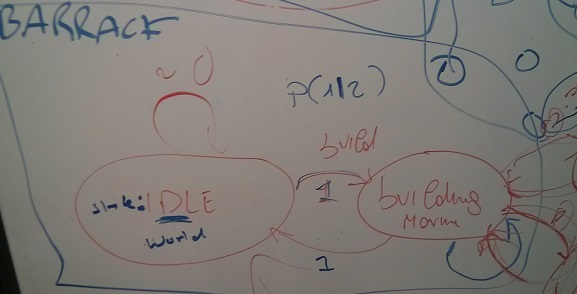
\includegraphics[scale=0.8, trim = 0cm 0cm 0cm 0cm]{diagrams/barracks}
\label{fig:barracks_diagram}
\caption{Markov Chain for unit building structures.}
\end{figure}

\subsection{Research Orientated Structures}

-create a similar generic diagram for research structures

-indicate using states how certain options are cut off


\section{Results}

%-what did we achieve?\\
% *managing scv units harvesting and building using Markov chains\\
% *system for buildings to train units using Markov chains

\begin{figure}[ht]
\centering
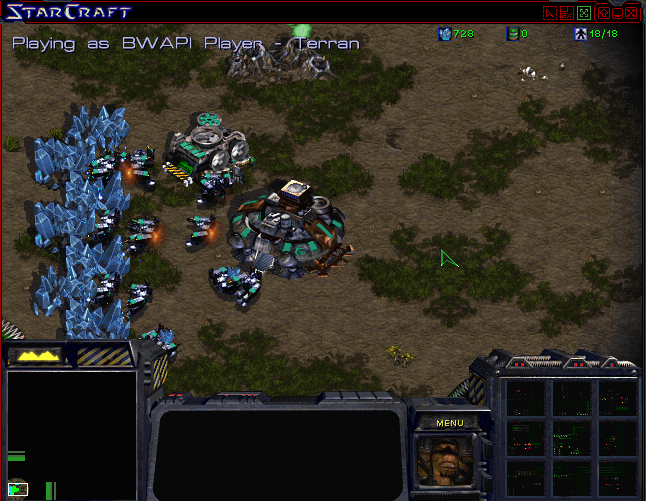
\includegraphics[scale=0.6, trim = 0cm 0cm 0cm 0.0cm]{images/Victory}
\label{fig:gameplay}
\caption{A screenshot of our agents gathering resources and some of the buildings they have constructed.}
\end{figure}


In the end we had a system for controlling SCV units and buildings using Markov chains which were influenced by the currently available unit slots and resources. Managing the splitting the SCV units between constructing buildings and harvesting and the point at which buildings created units were controlled by parameters the system could learn. The unit and base constructing and resource gathering aspects of the game could all be handled using Markov chains. Figure~\ref{fig:gameplay} shows an early stage of the game where SCVs are harvesting and have built a few buildings.

%-have we any way of evaluating our performance?\\
% *number of units and buildings completed after n-minutes?\\
% *needs to be somehow combined with a full strategy for proper evaluation (more in conclusion)..

 The problem we encountered was trying to decide on a way of evaluating the performance of our bot. The number and type of buildings and units on it's own is not a great performance metric. It would just result in the bot converging on optimum parameters to satisfy what is considered the best.

 The system could be paired with another agent to handle offensive capabilities but then the solution would choose optimum values for that bot and maybe even a specific enemy.

 Another method would be to compare the time at which we reach certain research levels and the unit output of our bot against the time that of other bots take to do the same.


\section{Conclusion}

%conclusions
-what do we think about the results?

-Difficulty in testing performance
 *evaluating building and resource gathering not straight forward\\
 *what is an optimal result of this process (speed in building attack units?)\\
 *how to test against other systems\\

-Needs integration with a full strategy to yield good results\\
 *would need testing against a multitude of bots to avoid over-training\\
 *different attack strategies could benefit from different Markov chains - would need to train for specific strategies.\\

%Future Work
Future work -other forms of learning algorithms?


-genetic algorithms\\
 + handle a multitude of different variables\\
 + could keep \textit{dna} binary strings separate for different agents and have agent specific genetic functions\\
 - would require many iterations to yield good results\\
 - performance metric operator still an issue

%%%%%%%%%%%%%%%%%%%%%%%
% sample figure code
%%%%%%%%%%%%%%%%%%%%%%%
%\begin{figure}
%\centering
%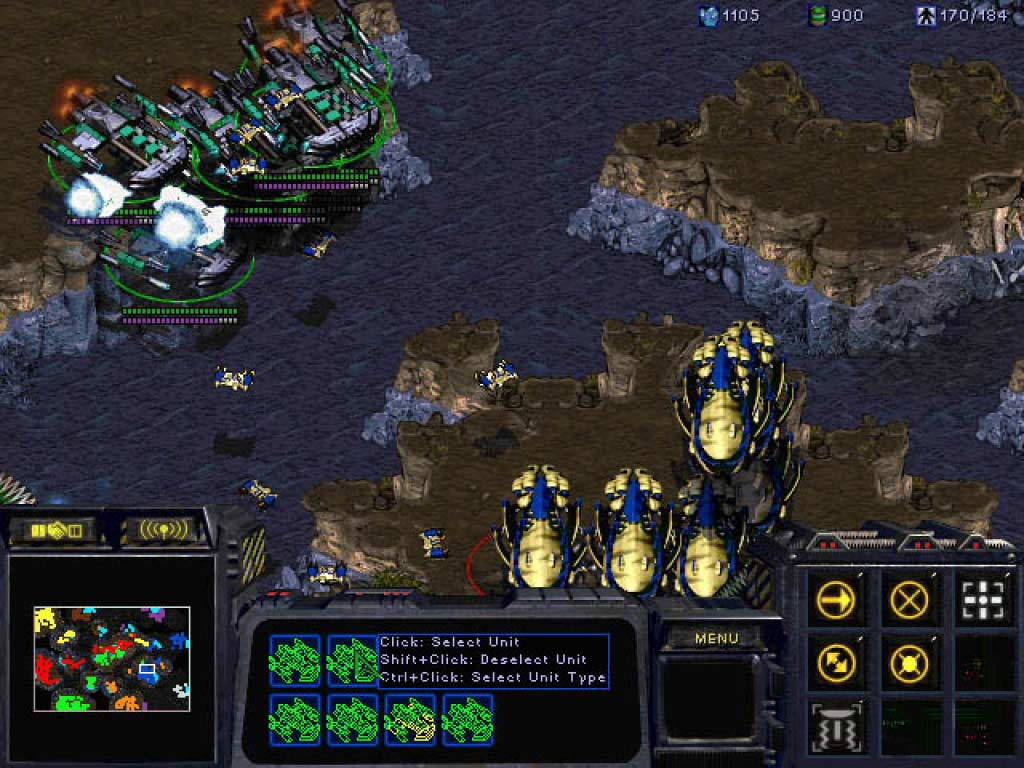
\includegraphics[scale=0.8, trim = 0cm 0cm 0cm 0cm]{images/test}
%\label{fig:some_label}
%\caption{some figure}
%\end{figure}


\newpage
\bibliographystyle{plain}
\bibliography{bibliography}
\label{endpage}


\end{document}




















